\section{Transition Pieces}
\label{sec:transitions}

Often it is necessary to have transitions in the beam pipe which can not be tapered, either due to space constraints or the operational requirements of the device containing the transition. This a common requirement in devices that require some mechanical freedom, such as bellows, or electrical isolation from the beam pipe, such as kicker magnets. For these devices it is often possible to use a transition piece, that is a one or several pieces of conducting material to screen any transition. These may be rigid or moveable as shown in Fig.~\ref{fig:rf_fingers}, often referred to as RF fingers.

\begin{figure}
\begin{center}
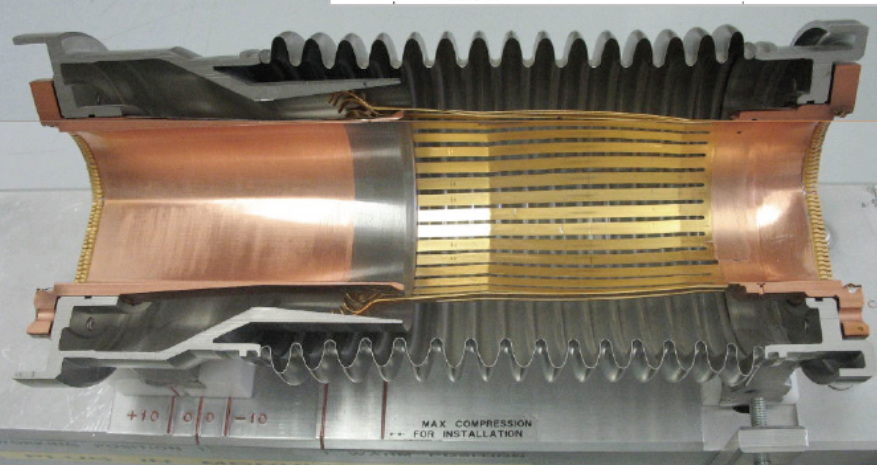
\includegraphics[width=0.45\textwidth]{Beam_Coupling_Impedance_Reduction_Techniques/figures/pimsImage.png}
\label{fig:rf_fingers}
\end{center}
\caption{Example of \ref{fig:rf_fingers} RF fingers (in this case for the PIMS module, placed between cryo-modules in the LHC).}
\end{figure}


This method of impedance reduction is effective for a number of reasons. Firstly it provides a short, good conducting path for the image currents to flow that does not expose it to the cavity created by the transition. This serves to reduce the broadband impedance increase due to the transition. Secondly, by correctly designing the spacing in the transitions, it is possible to minimise field leakage to the surrounding cavities therefore decreasing the visibility of cavity resonances. As an example of a cavity with and without RF fingers and a number of intermediatary steps, see Fig.~\ref{fig:rf_finger_imp}, which illustrates the case of the VMTSA, a vacuum interconnect in the injection region of the LHC \cite{Salvant:VMTSA}. It is characterised by a large vacuum chamber (due to needing to contain two circulating beams) with a long set of bellows. They were screened by a long set of RF fingers, which functioned well when good surface contact was maintained between the fingers and the beam pipe. However, when this connection was disrupted (easily created via mechanical stress due to the weak pressure exerted by the afixing spring).


\begin{figure}
\subfigure[]{
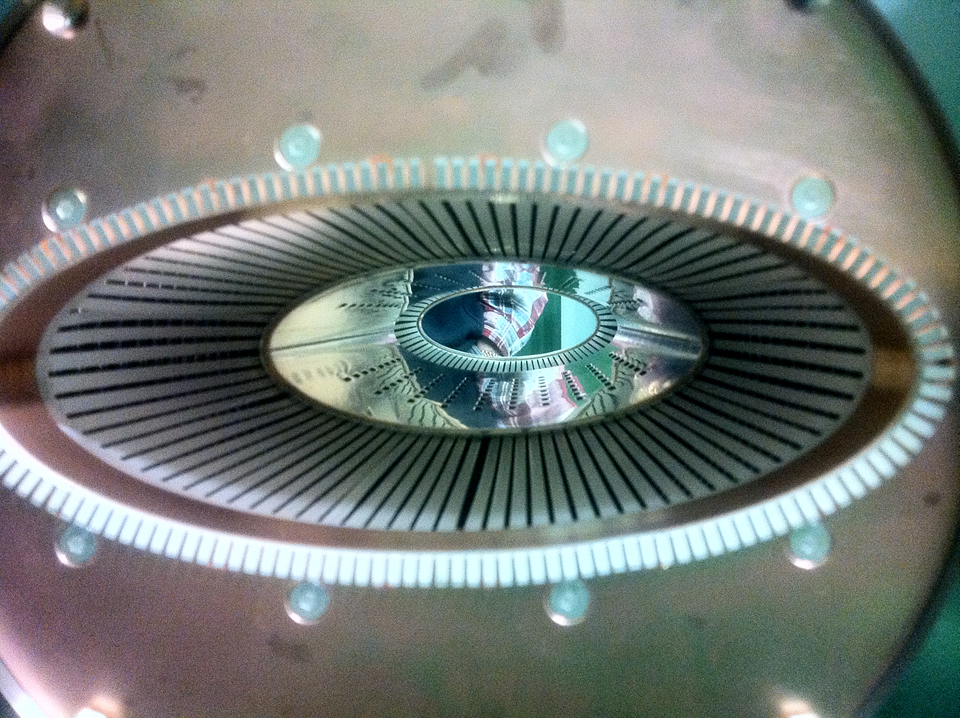
\includegraphics[width=0.3\textwidth]{Beam_Coupling_Impedance_Reduction_Techniques/figures/vmtsa-good-contact.png}
\label{fig:vmtsa_operations}
}
\subfigure[]{
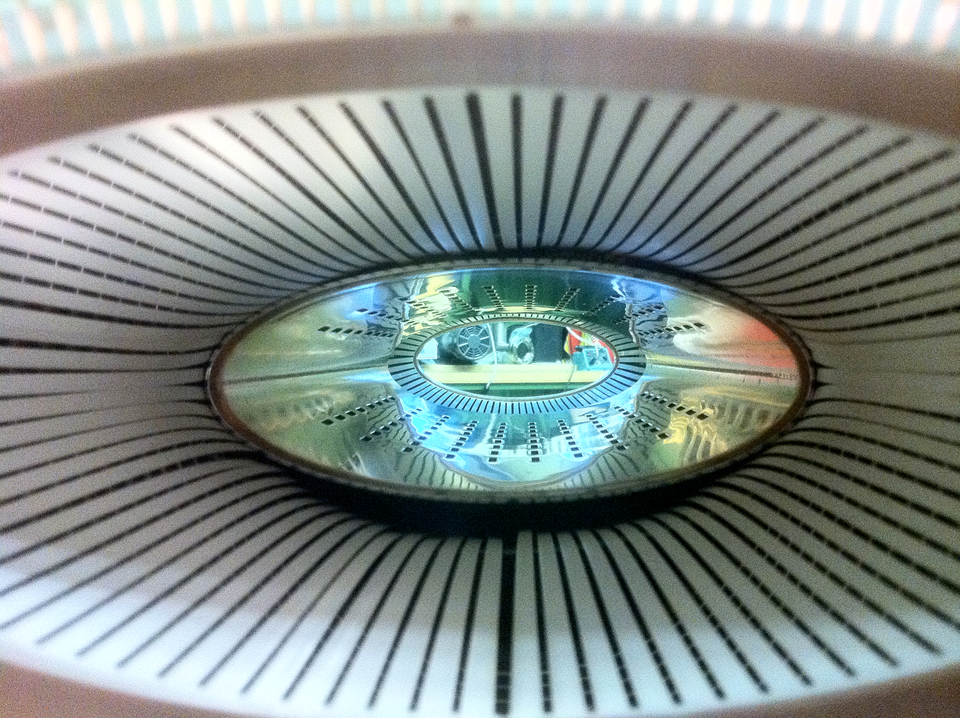
\includegraphics[width=0.3\textwidth]{Beam_Coupling_Impedance_Reduction_Techniques/figures/vmtsa-bad-contact.png}
\label{fig:vmtsa_failure}
}
\subfigure[]{
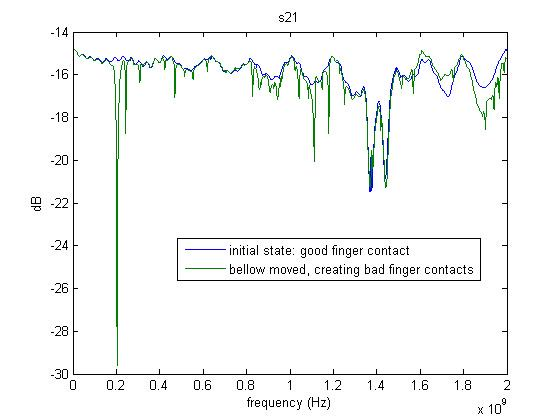
\includegraphics[width=0.3\textwidth]{Beam_Coupling_Impedance_Reduction_Techniques/figures/vmtsa-impedance.png}
\label{fig:vmtsa_impedance}
}


\label{fig:rf_finger_imp}
\caption{The layout of the RF fingers in the VMTSA both in \ref{fig:vmtsa_operations} the fully operational configuration and \ref{fig:vmtsa_failure} when the RF fingers lose contact. \ref{fig:vmtsa_impedance} shows the resulting beam coupling impedance of the two types of impedance as acquired by coaxial wire measurements. Photoes and measurements courtesy of J.L. Nougaret.}
\end{figure}